\documentclass[10pt]{article}
\usepackage{mathtools}
\usepackage{amssymb}
\usepackage{enumitem}
\usepackage[left=1.5cm, right=2cm, top=1cm, bottom=2cm]{geometry}
\usepackage{tikz}
\usepackage{graphicx}
\graphicspath{ {./images/} }
\usetikzlibrary{arrows,shapes,automata,petri,positioning,calc}
\setlength\parindent{0pt}
\title{Agile Recap - Answers/Summary}
\date{}
\author{}
\newcommand*\circled[1]{\tikz[baseline=(char.base)]{
            \node[shape=circle,draw,inner sep=2pt] (char) {#1};}}
\newcommand{\caselist}[1]{\begin{enumerate}[label=\protect\circled{C\arabic*}]#1\end{enumerate}}
\newcommand*{\true}{\circled{V}}
\newcommand*{\false}{\circled{F}}
\newcommand\xeq[1]{\,\stackrel{\mathclap{\normalfont\mbox{\tiny{#1}}}}{=}\,}

\begin{document}
\maketitle
Agile principles
\begin{itemize}
\item Put customer at the center
\item Let team self-organize
\item Work at a sustainable pace
\item Develop minimal software (functionality, only product requested, only code \& tests)
\item Accept change
\end{itemize}
\begin{itemize}
\item Develop iteratively (Frequent working iterations, freeze reqs during iterations)
\item Treat tests as key resource (No new development with failing tests, Test first)
\item Express Reqs. through scenarios
\end{itemize}
Practices
\begin{itemize}
\item Daily meeting\\
Coordinate 24hrs team plan, raise blockers. What did you do? what will you do? any blockers?. Around 15 min, no technical discussion allowed
\item Planning game/poker\\
Onsite customer/PO prioritizes stories, developers estimate them, game finishes when all agreed on estimate
\item Continuous Integration\\
Reduce tech debt by bringing together software/product components frequently. Automated build detects integration errors.
\item Retrospective\\
What went well? What went less well? How do we improve? Team + coach (SM), PO can attend
\begin{enumerate}
\item Brainstorm subjects to improve
\item Vote on highest priority improvement
\item Do short analysis
\item Create improvement story, place it atop next sprint backlog
\item Schedule Problem Solving Workshop if necessary
\end{enumerate}
\item Shared code ownership \& cross-functional teams - it's lower down in this file
\item TDD, Refactoring also lower down
\end{itemize}
XP Values
\begin{itemize}
\item Communication - everyone on team works jointly on all stages
\item Simplicity - write simple code
\item Feedback - deliver frequently \& get feedback on reliveries
\item Respect
\item Courage - Evaluate own results without making excuses, be ready to respond to change
\end{itemize}
XP Principles
\begin{itemize}
\item Rapid Feedbvack - Team members understand and respond to feedbvack
\item Assumed simplicity - Follow YAGNI and DRY
\item Incremental changes - Small changes to the product
\item Embracing change - if client requests changes, support the decision and plan implementing the reqs.
\item Quality work - Team works well, makes a valuable product, is proud of it
\end{itemize}
XP Practices
\begin{itemize}
\item Pair programming
\item Onsite-Customer
\item Test-first
\item Planning game
\item Feedback
\item Continuous process - Small releases, CI, Refactoring
\item Programmer welfare - sustainable pace
\item Shared understanding- Coding standards, Collective Code Ownership, System metaphor, simple design
\end{itemize}
Scrum roles
\begin{itemize}
\item Product Owner maximizes value added by owning and deciding on priorities in the Team Backlog from a business perspective. Maintains technical integrity of features + components
\item Dev teammember is part of cross-functional team accountable for providing value to the larger solutions/systems
\item Scrum master is a servant leader + coach that uses/enforces Agile practices (sprint planning, dailys, demos, retrospectives). Focus opn flow and continuous improvements
\end{itemize}
Product backlog
\begin{itemize}
\item List of prioritized things to be done
\item Continuously updates (never complete)
\item DEEP: Detailed appropriately, Emergent, Estimated, Prioritized
\end{itemize}
A product backlog is the aggregation of all the project backlogs pertinent to the product.
\begin{itemize}
\item Acceptance criteria: define scope of user story/feature/capability
\item DoR: List of criteria for a user story/features/capability to be pulled from backlog
\item DoD: Criteria to consider accepted
\end{itemize}
If stuck, reduce functionality and keep to the schedule, instead of trying to modify the schedule or add developers
\begin{itemize}
\item '9 pregnant women don't make a baby in a month'. Essentially, adding more developers rarely speeds up development in the short-term (can work long-term, but not relevant to this question)
\item K eeping to deadlines in timeboxed iterations/sprints ensures a predictable delivery cycle and workload
\item Lengthening development cycles reduces feedback from deliveries
\item Reprioritization helps deliver on critical features while allowing those that appear less essential to be deferred
\item Sustainable pace (No death marches or whatever)
\end{itemize}
Big upfront requirements, why Agile opposes them and why some are still beneficial
\begin{itemize}
\item Agile seeks adaptability, feedback, delivering value early
\begin{itemize}
\item Collecting big upfront requirements delays the start of development
\item Predefined requirements/product specifications hinder adaptability \& customer feedback
\item Embrace change
\item Working software over comprehensive documentation
\item Incremental + iterative approach
\item Reduce risk + waste
\end{itemize}
\item Some upfront planning is useful
\begin{itemize}
\item Define a product vision + goals, tech stack, etc. (As we did in Sprint 0)
\item Set architectural foundations. Concerns over scalability, security, and integration should be considered early on in a project
\item External dependencies, risk analysis, legal requirements, budgeting, stakeholders cannot be 'discovered iteratively'
\end{itemize}
\end{itemize}
Thinking on the video of the ping pong ball, establish a flow before optimizing resources.\\
Importance of having customer relations
\begin{itemize}
\item XP has a customer representative role within teams (This isn't very viable, but still you get the point)
\item Agile teams should have some role that interfaces with customers.
\item Not all customer feedback is great - Customers don't really know what they want much of the time
\end{itemize}
Kano model:\\
Graph satisfaction on y-axis, level of fulfillment on x-axis.\\
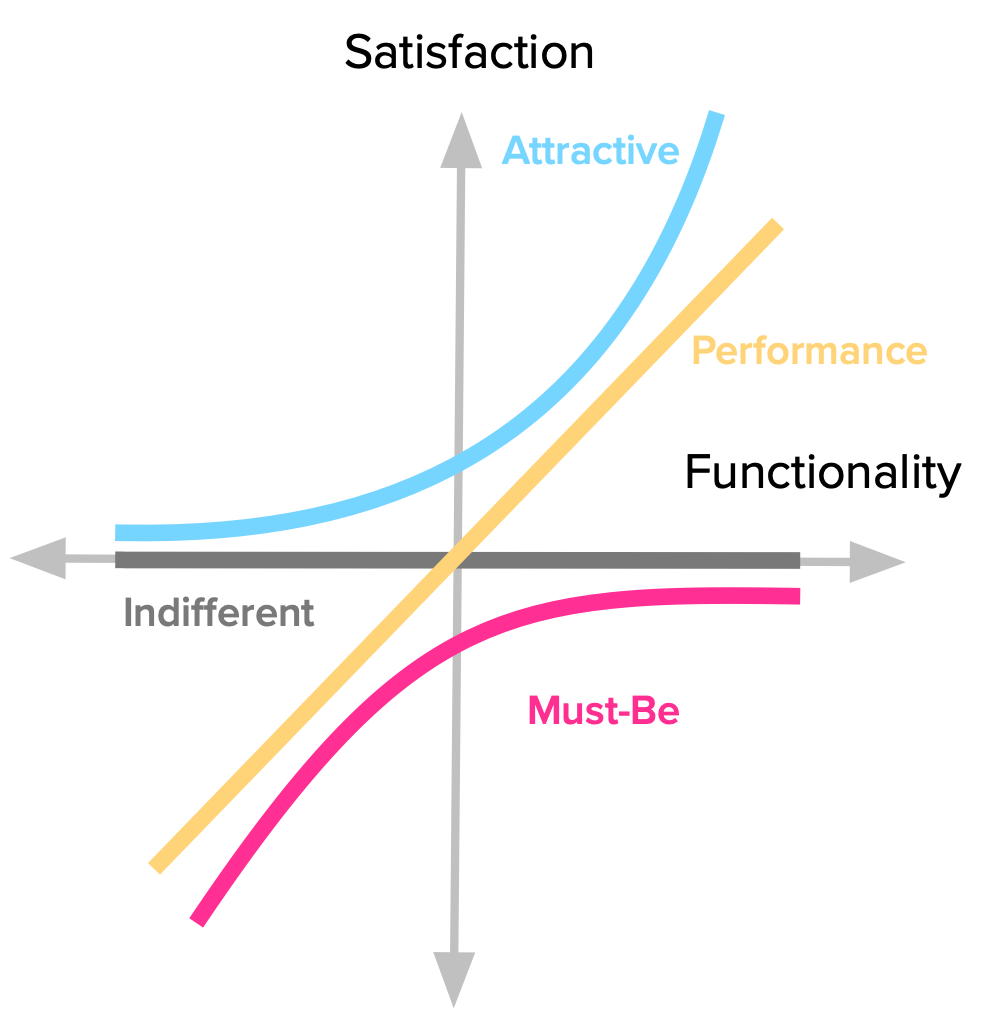
\includegraphics[width=5cm, height=5cm]{kano}\\
Projects/developers should be executed at a sustainable pace, sprints should be planned with cushions of leftover time for the team members in case of unforeseen obstacles\\
Additive vs Multiplicative complexity
\begin{itemize}
\item Additive complexity refers to the linear growth of software complexity that simply results from the growth of a codebase/product
\item Multiplicative complexity is often the result of a poorly designed architecture; increasing dependencies make it such that every additional feature multiplies the number of interactions, increasing complexity further
\end{itemize}
Accepting vs liking change
\begin{itemize}
\item I wouldn't dwell too much on this, the concept is self-explanatory
\item PMs don't really enjoy change, but as part of Agile teams they should be willing to expect and accept it
\end{itemize}
Weighted-shortest-job-first feature prioritization
\begin{itemize}
\item I vaguely remember there being a slide and a short exercise on this, there will be an exam question about it, I will probably not have read the slide because I don't wanna search for it, assuming the concept is self-explanatory and then realize I probably should have at least skimmed the slide.
\end{itemize}
Iterative development
\begin{itemize}
\item Small incremental improvements. Break work down into iterations (Sprints in Scrum), each should produce a shippable product increment. Deliver working software in small steps rather than delivering all at once
\item Frequent feedback and adaptation. Sprint review, demos, user testing are some of the feedback loops involved in iterations.
\item Continuous learning \& improvement. Retrospectives and learning on each cycle improve processes and decision-making
\item Value prioritization. Features are delivered based on business value, backlog is refined to reflect changing priorities
\item Reduced risk \& early problem detection
\end{itemize}
\begin{itemize}
\item In Scrum, iterations are defined as sprints (1-4 weeks) where a set of backlog items are developed and reviewed
\item In Kanban, Continuous iteration occurs through small batch delivery and WIP limits
\item In XP, there are frequent releases (sometimes multiple per day) with constant refactoring and feedback
\end{itemize}
Requirements vs Scenarios
\begin{itemize}
\item Requirements cover the complete scope of functionalities, user stories cannot replace these, as you can't fully define a specification with them
\item Sometimes requirements are necessary, think of legal requirements, architectural, performance, etc.
\end{itemize}
Scrum ceremonies
\begin{itemize}
\item Daily meeting
\item Sprint demo
\item Sprint planning
\begin{itemize}
\item Planning Poker
\end{itemize}
\end{itemize}
Shared code ownership \& cross-functional teams
\begin{itemize}
\item In shared code ownership, the entire team is responsible for all code, instead of having individual devs responsible for/'owning' sections
\item Cross-functional teams refers to teams with knowledge from different areas. The professor speaks of wanting 'T-shaped' team members in Volvo Cars, with expertise in one specific area but at least surface-level knowledge on the rest of the areas relevant to the project
\end{itemize}
\begin{itemize}
\item Shared code ownership can improve code quality by bringing more eyes to each piece of code, speed up development by reducing bottlenecks on specific devs, encourages knowledge sharing and makes refactoring easier (no approval from a specific dev)
\item Inconsistent coding styles, merge conflicts \& overwrites, reduced sense of ownership/accountability and a need for strong communication are some drawbacks of shared code ownership
\item Cross-functional teams can speed up delivery by reducing handoffs between teams, they improve collaboration and flexibility and are able to consider more aspects of a product, improving quality
\item Cross-functional teams can face challenges with coordination, conflicting priorities, skill gaps and scaling (managing cross-functional teams in large organizations is complex)
\end{itemize}
Personal thoughts on pair programming
\begin{itemize}
\item Personal preferences and different work ethics: should not be forced onto all developers 
\item XP likes it
\end{itemize}
Test-Driven Development - Know 5 steps in detail, be able to provide examples (our own work is relevant, mention the Unit tests we wrote with JUnit for our backend, be aware that we wrote those tests after implementing the feature though so maybe google a better example and write it down here please uwu)
\begin{enumerate}
\item Quickly add a test
\item Run all tests, see the new one fail
\item Make a small change
\item Run all tests again, see them succeed
\item Refactor \& remove duplication
\end{enumerate}
Extreme Programming (XP)\\
Practices - Please list them down here if you have the slide with them on you :D. We need to be able to explain them listing them by heart is not necessary though\\
I am starting to believe that this subject is not worth the 3 credits I'll be getting at my home uni\\
Also, someone tell the student representatives that is the professor wants to forego the exam but also ensure that we actually learn the contents while keeping the primary focus on the project then having us answer the questions to the exam by sections as group assignments throughout the project would be a very effective way of achieving this while also being much less of a pain in the big O for all of us.
\begin{itemize}
    \item Pair Programming 
    \item System Metaphor
    \item Shared Code Ownership
    \item Small Releases
    \item Simple Design
    \item 40 Hour Week
    \item Planning Game
    \item Coding Standards
    \item Test first
    \item Continous Integration 
    \item Customer On-site
    \item Refactoring
\end{itemize}
\begin{itemize}
\item Product Owner: customer representative, owns the product backlog, ensures team is building the right thing, prioritizes items in the product backlog, must also be able to negotiate and say "no" to the customer
\item Scrum Master: Servant Leader ensures good working environment for the development team and removes impediments, coaches, initializes the agile ceremonies
\item Development Team: self-organized cross-functional team, commits to delivering items in the sprint backlog, T-shaped team
\end{itemize}
Product backlog, why it should be detailed, what a DEEP backlog is, why we want ONE product backlog\\
Difference between project and product\\
User stories, INVEST format
\begin{itemize}
\item Independent
\item Negotiable
\item Valuable
\item Estimable
\item Small
\item Testable
\end{itemize}
Be able to break down a functionality into around 10 user stories:\\
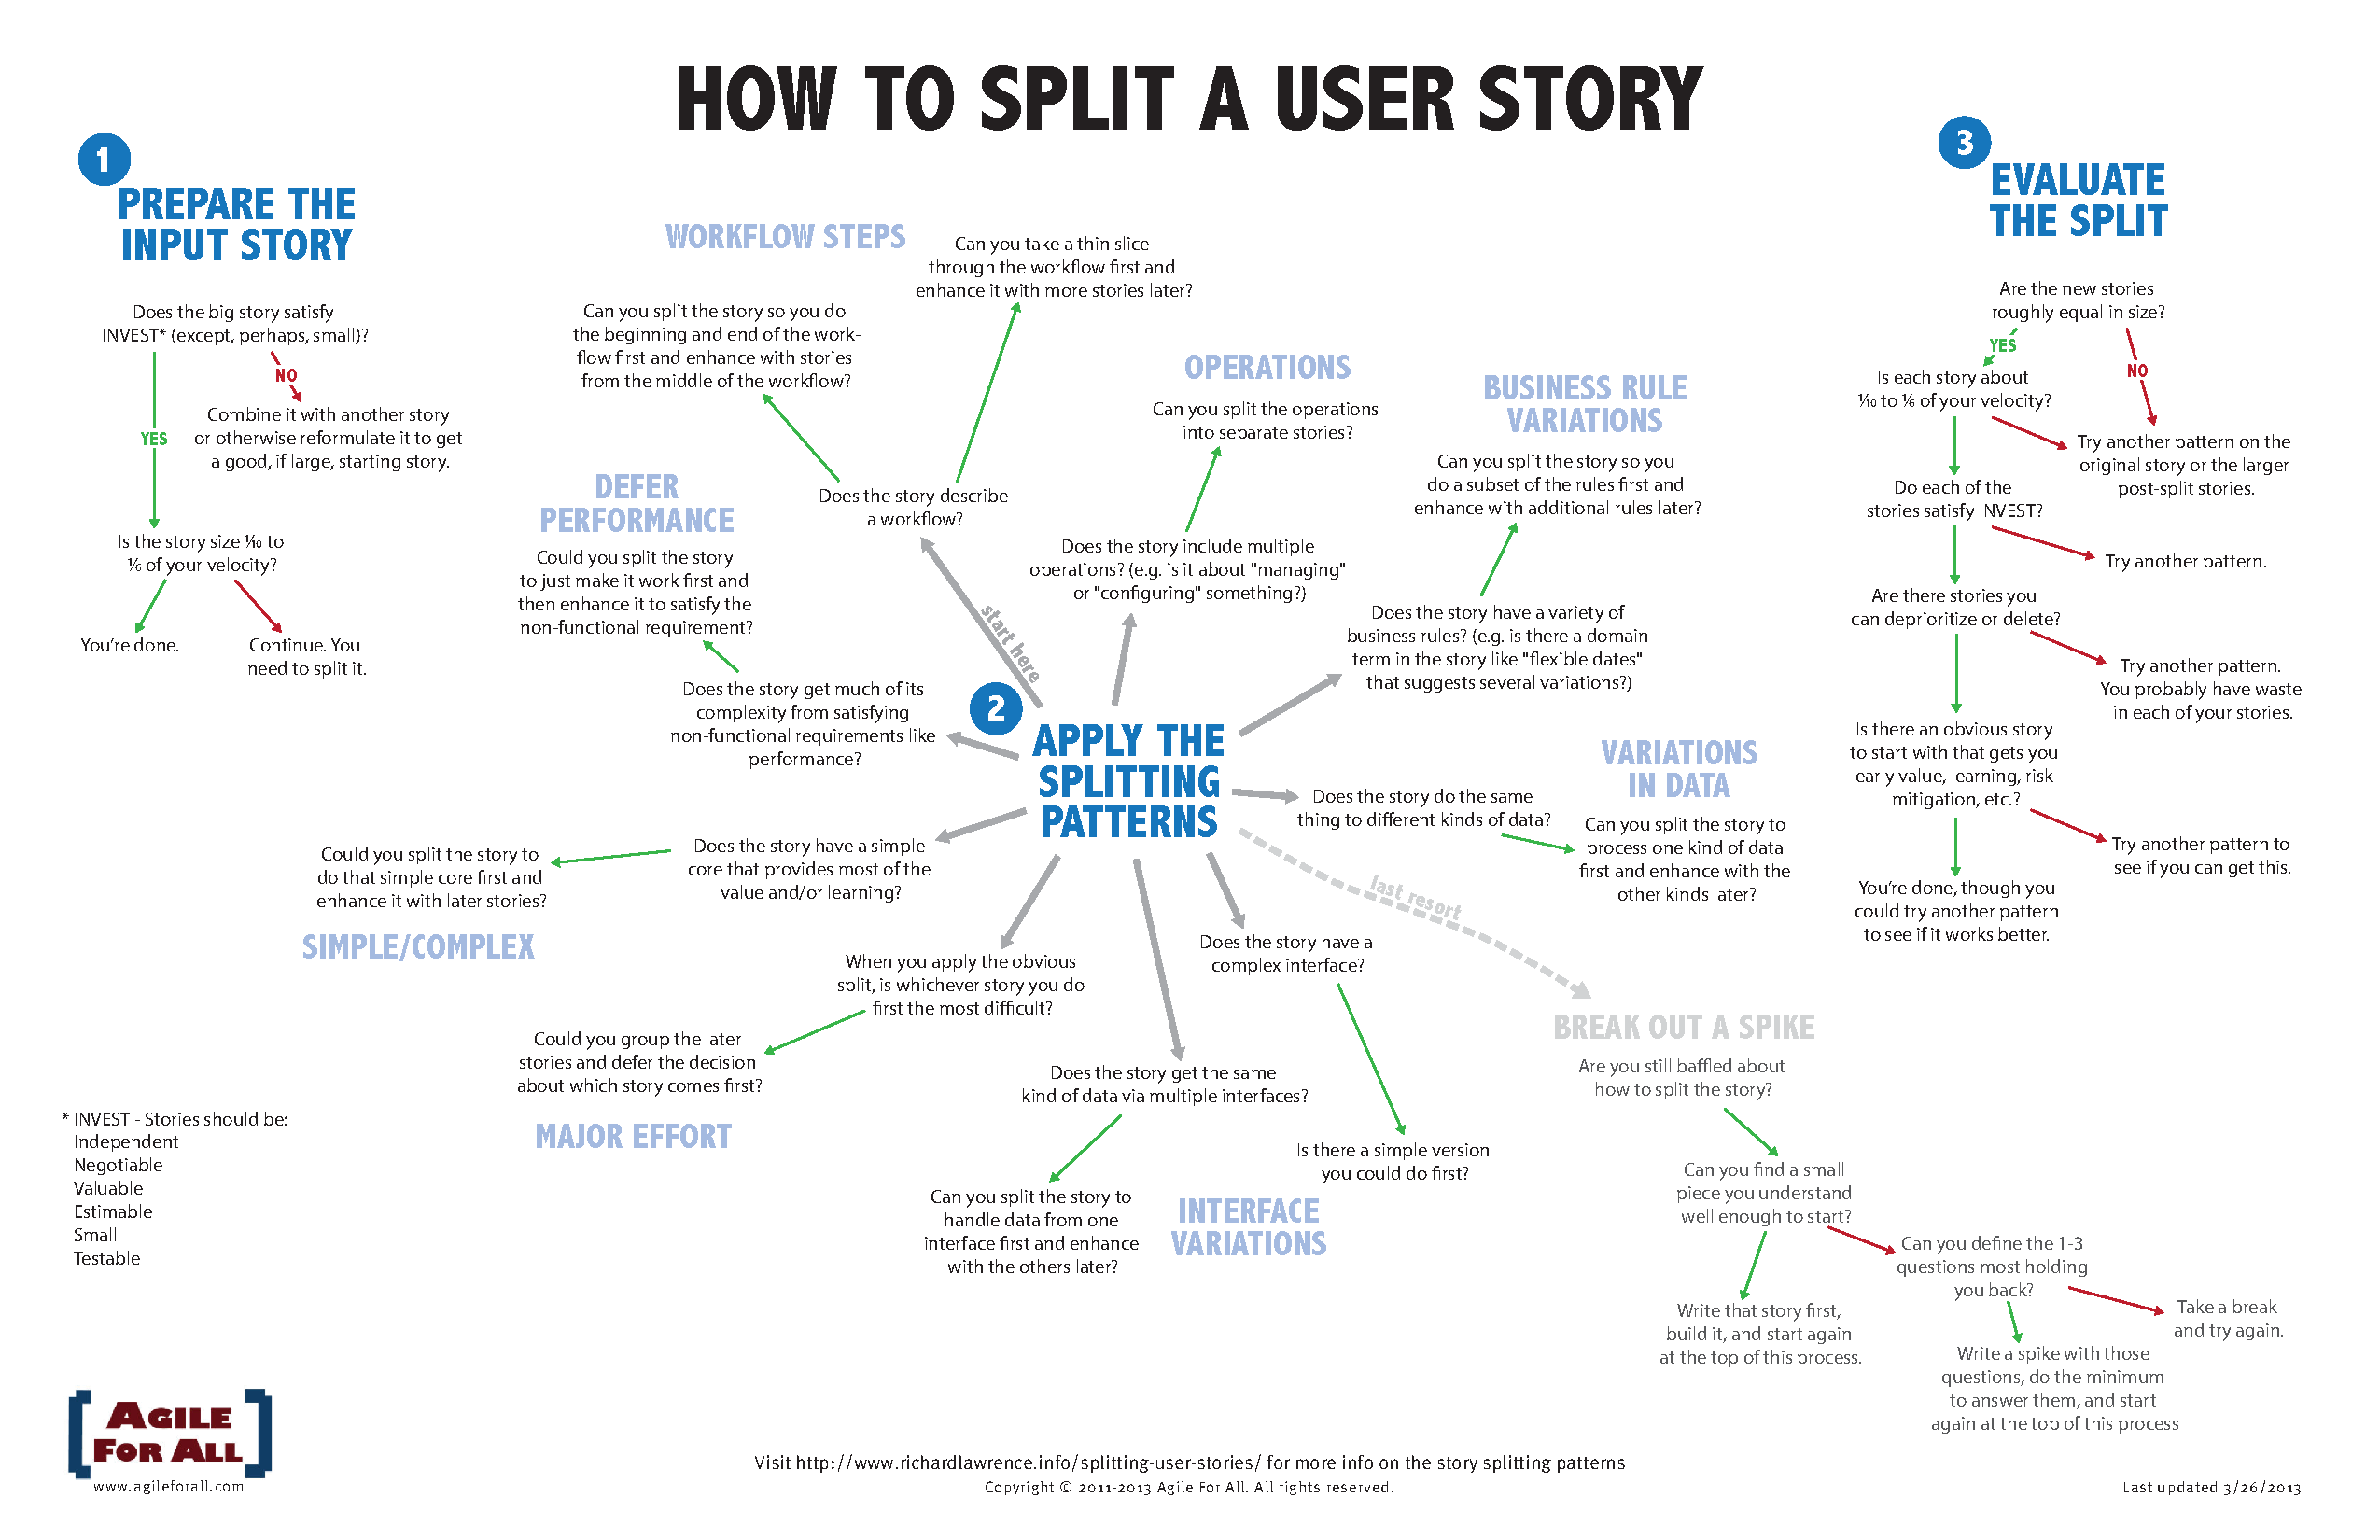
\includegraphics[width=12cm, height=10cm]{userstories-flowchart}\\
Functional vs Non-functional requirements
\begin{itemize}
\item Functional:
Define what the system should do
Independent, Negotiable, Valuable, Estimatable, Small, Testable
\item Non-functional:
Define the constraints and how the system should behave
Bounded, Independent, Negotiable, Testable
\end{itemize}
Enable stories refer to technical needs, architectural improvements, or infrastructure required to deliver normal user stories. Normal user stories describe functionality/scenarios that deliver value to the customer\\
Capacity expresses an amount of work that can be done given a space of time, velocity refers to the amount of work that has been done in a space of time\\
Be able to explain a proposed-job allocation as PO or SM\\
Story points are estimations of the amount of effort (sometimes time) required to complete an element in a backlog (usually user story/task)\\
Sprint 0 is a preliminary sprint often added on Scrum methodologies for dealing with architectural/tech stack planning, definitions of DoD, product vision, etc. (all those small big upfronts we all hate)\\
Burnup and Burndown charts, watch a slide idk\\
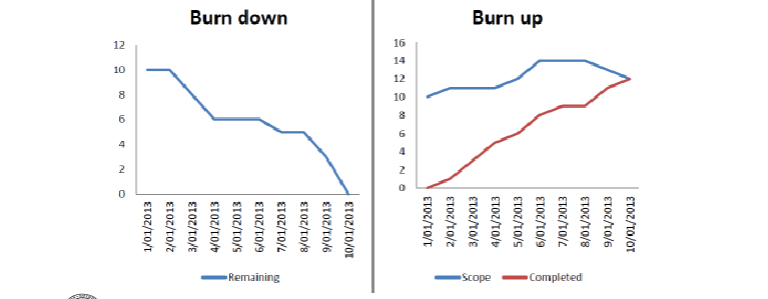
\includegraphics[width=10cm, height=5cm]{Burndown}\\
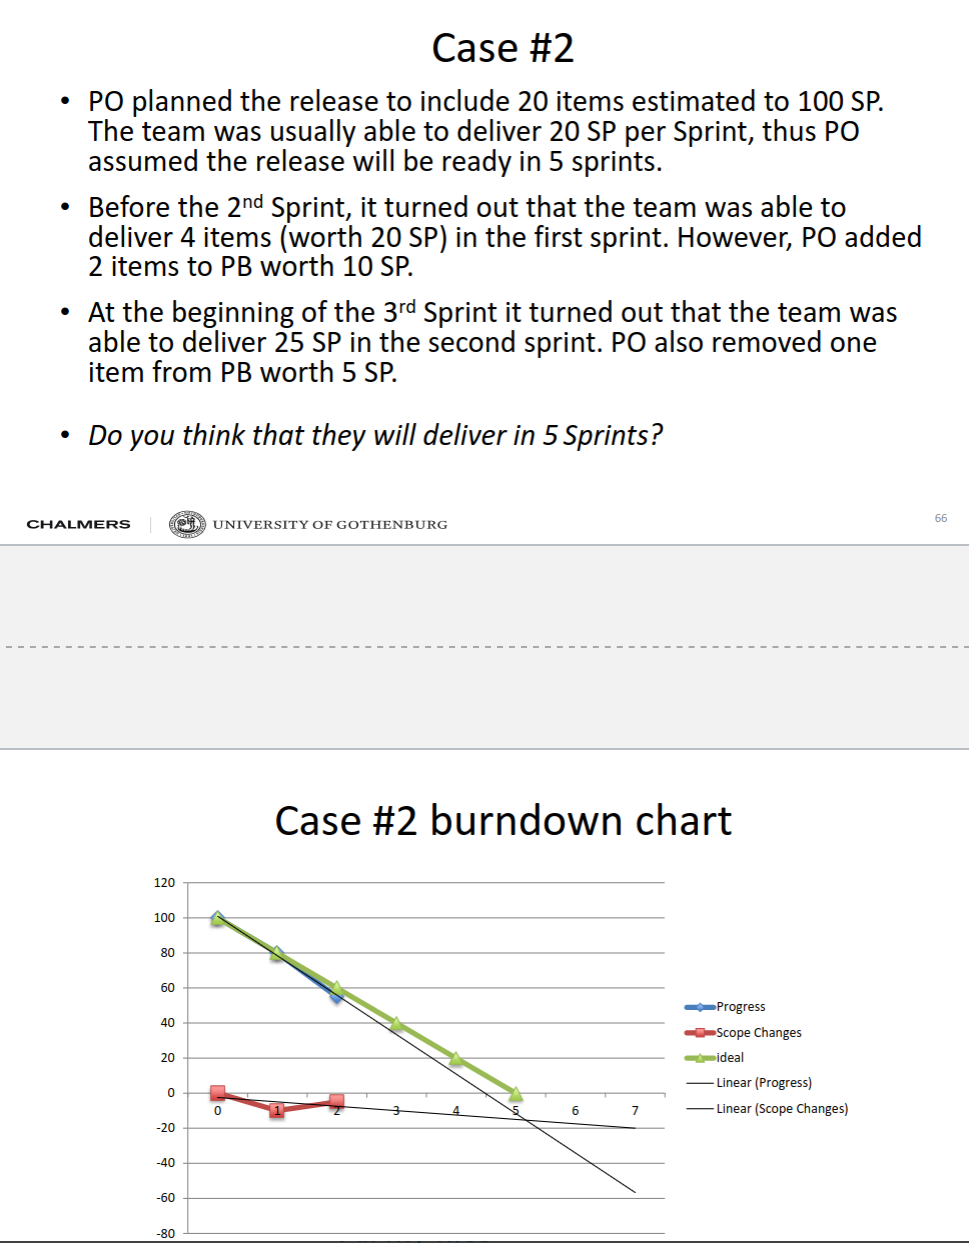
\includegraphics[width=10cm, height=15cm]{Burndown2}\\
Lean originates in manufacturing, Scrum in software dev.\\
Lean principles:
\begin{itemize}
\item Eliminate waste:\\
Tool: \begin{enumerate}
\item Inventory/partially done work
\item Extra processing - paperwork
\item Over production - unused features
\item Transportation - task switching
\item Waiting - staffing, approval, review, excessive reqs., testing, deployment
\item Motion - handovers, finding answers to questions
\item Defects
\end{enumerate}
Tool: Value Stream Mapping\\
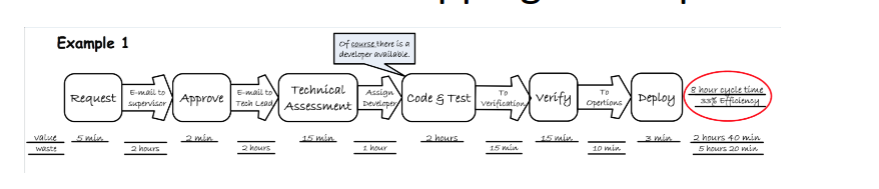
\includegraphics[width=16cm, height=4cm]{VSM}
\item Amplify learning - Incorporate feedback from dev, tests, retrospectives, etc. into development process\\
Tool: Feedback\\
Tool: Short iterations; increase control, help sync devs and customer, force decisions to be made\\
Tool: Synchronization: Daily scrum, build, system test, weekly push to master, weekly meetings (scrum-of-scrum)
\item Decide as late as possible\\
Keep options open as long as is practical, allows you to survey landscape, delay detailed decisions, breadth-first development allows managing risk\\
Tool: Last responsible moment - that in which failing to make a decision eliminates an important alternative
\item Deliver as fast as possible: Limit WIP by delivering fast, faster delivery increases customers' business flexibility, prevents them changing their minds, keeps resources from getting tied up in WIP. The faster you deliver, the longer you can delay decisions\\
Tool: Pull system; every team member knows how to contribute best, everyone sees what's going on, what needs to be done, what problems exists, what progress is being made\\
Tool: Queuing theory; Cycle time is the measurement of a queue, minimize cycle time. Consider arrival rate, service rate, resource load\\
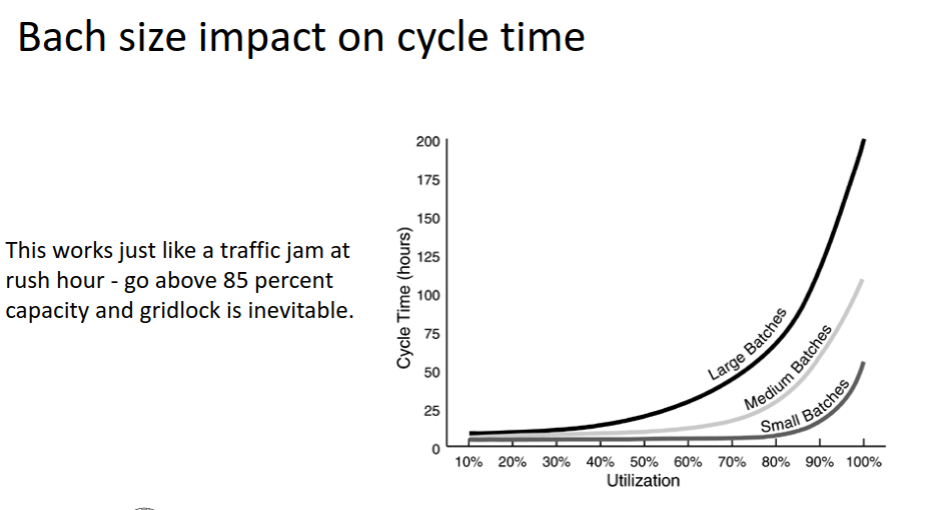
\includegraphics[width=10cm, height=8cm]{Batch}\\
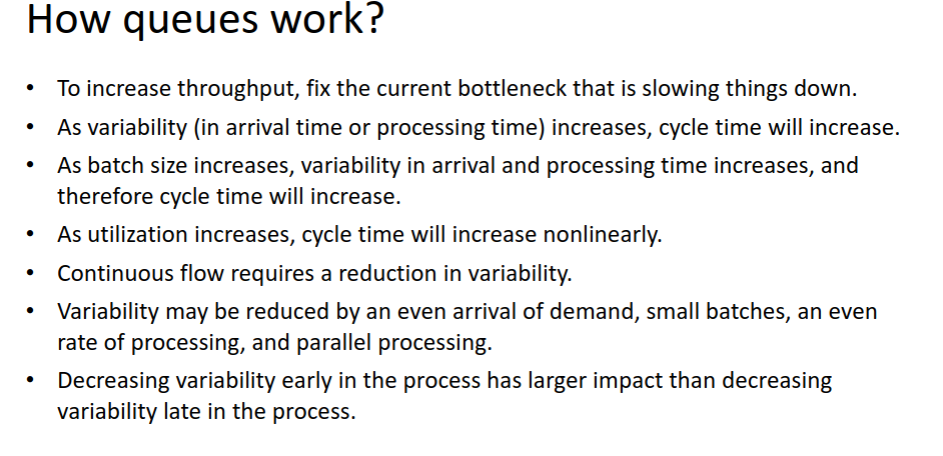
\includegraphics[width=10cm, height=8cm]{Queue}\\
Tool: Cost of delay; from an economic model, show how revenue and market share affect profits in relationship to delays
\item Empower the team: Move decisions to the lowest level possible while developing the capacity of those people to make decisions wisely\\
Tool: Leadership
\item See the whole: Software systems are not just the sum of their parts, but the product of their interactions. Avoid local sub-optimization\\
Tool: Contracts
\end{itemize}
Lean process:
\begin{enumerate}
\item Identify value
\item Map value streams, visualize with Kanban board\\
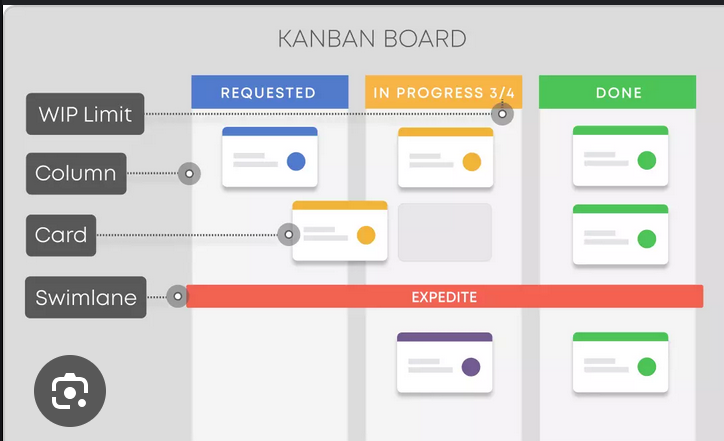
\includegraphics[width=10cm, height=8cm]{KBoard}
\item Create flow, limiting WIP
\item Establish pull from common prioritized backlog, clear rules for moving tasks in Kanban board
\item Seek perfection, constantly remove waste
\end{enumerate}
Agile focuses on local-level communication, Lean advocates holistic view of delivery change, XP advocates 'decide now, change later', Lean defers commitment
Global optimization\\
Value Stream Mapping + Know how to improve the efficiency of a given development process\\
'Last responsible moment' for decision making\\
Queuing theory
\begin{itemize}
\item Arrival rate
\item Service rate
\item Resource load
\end{itemize}
How small vs large batches pass through the process, diagram showing how batch size affects cycle time.\\
Difference between Lean, Agile, Kanban, XP, etc.\\
Kanban
\begin{itemize}
\item Pull system that visualizes workflow and uses WIP to facilitate flow
\item The Kanban board
\item Kanban phases
\end{itemize}
Kanban principles
\begin{itemize}
\item Start with what you do now
\item Agree to pursue incremental evolutionary change
\item Respect current process, roles, responsibility, titles
\item Leadership at all levels
\end{itemize}
Kanban Practices
\begin{itemize}
\item Visualize workflow to understand \& improve
\item Limit WIP
\item Manage flow
\item Make policies explicit
\item Implement feedback loops
\item Improve collaboratively, evolve experimentally - whole team shares theory on why small change helps
\end{itemize}
Scrumban, which aspects of each can be integrated in what scenarios. Read through Lecture 4 table on SCrum vs Kanban\\
Lean focuses on frequent deliveries and quality, XP deals with these aspects indirectly\\
Kaizen - Continuous improvement\\
Agile leadership, the triangle of FUNCTIONALITY, TIME, COST ( + QUALITY)\\
A manager should provide for their teams:
\begin{itemize}
\item Autonomy
\item Master
\item Purpose
\end{itemize}
Concept of less is more, one example is not focusing on elements of little value, pick off the 'low-hanging fruit' that offers the most instant value rather than prototyping and planning endlessly\\
Be able to decide \& justify what features you would promise to a customer given some tasks, velocities, etc.\\
forming, storming, norming, performing\\
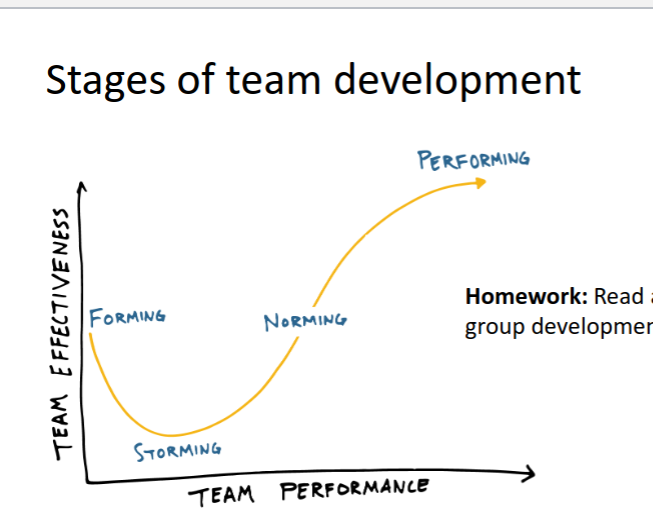
\includegraphics[width=8cm, height=8cm]{development}\\
Servant leader vs regular leader. Encourages ideas rather than giving answers, builds trust, is people-focused. Encourages team members to find own answers to questions, enables them and provides required resources.\\
Levels of authority
\begin{enumerate}
\item Tell
\item Sell
\item Consult
\item Join
\item Advise
\item Confirm
\item Delegate
\end{enumerate}
Look at the video on the submarine captain, reflect on leadership styles, what we can gain from each of them. Products should be busy, rather than team members \\
Concept of the sphere of influence, don't focus on things you have little impact on\\
Cynefin framework. Categorizes problems into domains
\begin{itemize}
\item Obvious - identify issue, apply a proven solution
\item Complicated - analyze problem, consult experts, find best solution
\item Complex - probe, sense, respond: experiment, gather feedback, adapt
\item Chaotic - Act, sense, respond: Take immediate action to stabilize, then find solutions
\item Disorder - Break problem down into the other four domains
\end{itemize}
Types of reporting, state vs. prognosis. How would you report a status to your manager?\\
Change curve\\
How commitment impacts predictability and productivity. Why teams should not overcommit (Agile advises working at a sustainable pace, no death marches, avoid burnout, etc.)\\
5 dysfunctions of a team - Will not be asked I can't be arsed\\
Random stuff about guest lecture: How would you work/what tools would you use if you worked in a team like the lecturer's?\\
Unit, Integration, System, Acceptance testing
\begin{itemize}
\item Unit testing refers to tests for specific elements/methods/functions of an interface
\item Integration testing refers to testing that involves bringing together 2 or more parts of a system and testing that they work together correctly
\item System testing involves building a software application as a whole and testing it against a set of requirements
\item Acceptance/end-user testing refers to determining whether an application meets end-users' approval
\item Software in the Loop testing refers to testing software in a simulated environment before integrating with real hardware
\item Hardware in the Loop testing refers to hardware testing in a real-time simulated environment 
\end{itemize}
A regression test suite is the selection of test cases used to ensure added code/features do not cause a regression (error/loss of functionality)
A regression test then is a test in the regression test suite\\
Principles of continuous integration
\begin{itemize}
\item 
\end{itemize}
Single source of truth/information for the software product, defined pulling and merging procedures\\
Version vs revision vs branch vs baseline
\begin{itemize}
\item Configuration item: file/document
\item Version: sequentially stored chagnes of configuration item
\item Revision: change to document's contents
\item Branch: changes in configuration item isolated from other cahnges
\item Baseline: specific version of each CI at a certain occasion, can be used as logical basis for test/release
\end{itemize}
\begin{itemize}
\item 
\end{itemize}
Test prioritization
\begin{itemize}
\item Usually done statistically based on the set of tests that commonly fail in relation to modifications in the given component of the product.\\
Collect which modules/components were changed, sort tests by fail frequency in connection to these changes/modules, choose a cutoff criteria for the ranked test list
\end{itemize}
Delivery vs deployment
\begin{itemize}
\item Deployment refers to ensuring the product is functional \& can be downloaded/accessed instantly 'with one click', delivery refers to the actual ct of the customer receiveing and installing software
\end{itemize}
Continuous Delivery vs Continuous Deployment
\begin{itemize}
\item 
\end{itemize}
Deployment practices (Name at least 3)
\begin{enumerate}
\item Dark launching
\item Feature flag
\item Rollouts
\end{enumerate}
DevOps, conflicts, why prod and dev. environments should not be different
\begin{itemize}
\item DevOps = development + operations
\item Automate everything, identical dev \& deployment environments, Source control system, performance monitoring, \& optimization in real time, measure everything
\end{itemize}
CI principles
\begin{itemize}
\item Maintain Single Source Repository
\item Small and Frequent Commits
\item Fail fast, fix fast
\item Follow your commit
\item Automate the flow
\item Everyone can see what's happening
\end{itemize}
CI practices
\begin{itemize}
\item Don’t check in on a broken build
\item  Always run all commit tests locally before committing (if not your Ci
server does it for you)
\item Wait for commit test to pass before moving on
\item Never go home on a broken build
\item Always be prepared to revert to previous revision
\item Time-box fixing before reverting
\item Don’t comment out failing tests
\item Take responsibility for all breakage that result from your changes
\item Test driven development 
\end{itemize}
SAFe (Scaled Agile Framework) Principles
\begin{enumerate}
\item 
\end{enumerate}
SAFe\\
Implementation roadmap\\
Group manager vs Team manager
\begin{itemize}
\item 
\end{itemize}
Product Increment (PI) Planning
\begin{itemize}
\item 
\end{itemize}
Agile Release Train
\begin{itemize}
\item 
\end{itemize}
Develop on a cadence, release on demand\\
Solution train engineers, solution managers, system architects
\begin{itemize}
\item 
\end{itemize}
Architectural runway/runaway
\begin{itemize}
\item The scope of features/functionalities that can be built on the product on the current architecture (the runway)
\end{itemize}
Conflict between Product and Solution management (PM and System Architect)
\begin{itemize}
\item 
\end{itemize}
Decentralizing decisions between interfaces
\begin{itemize}
\item 
\end{itemize}
Shared services \& system team outside ART
\begin{itemize}
\item 
\end{itemize}
Backlogs and roles on different levels of the framework. Epics are broken down into Capabilities, Capabilities into features, features into stories\\
Define 'the visions' of a company given its product (what kind of snake oil salesman shit is this)

product refers to an ongoing offering/service that provides value to userse, it is continuously improved, sold, maintained. A project refers to a temporary effort to create a specific deliverable within a timeline, scope, budget
\end{document}
